\documentclass[tikz,border=4mm]{standalone}
\usepackage{amsmath}
\usepackage{tikz}
\usetikzlibrary{automata,arrows,positioning,calc}
\begin{document}

\begin{center}
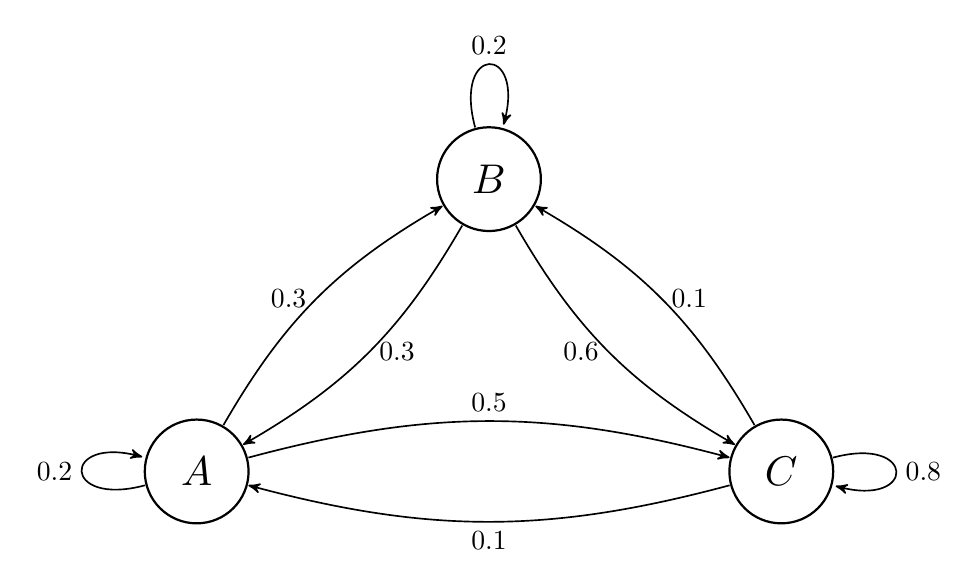
\begin{tikzpicture}[->, >=stealth', auto, semithick, node distance=3.5cm]
\tikzstyle{every state}=[fill=white,draw=black,thick,text=black,scale=1.5]
\node[state]    (A)                     {$A$};
\node[state]    (B)[above right of=A]   {$B$};
\node[state]    (C)[below right of=B]   {$C$};
\path
(A) edge[loop left]                 node[left]{$0.2$}         (A)
    edge[bend left=15]              node[above,left]{$0.3$}     (B)
    edge[bend left=15,below]        node[above]{$0.5$}      (C)
(B) edge[bend right=15,below]       node[below,left]{$0.6$}           (C)
    edge[bend left=15,below]        node[below,right]{$0.3$}              (A)
    edge[loop above]                node{$0.2$}              (B)
(C) edge[loop right]                node[right]{$0.8$}     (C)
    edge[bend right=15,right]       node[above,right]{$0.1$}      (B)
    edge[bend left=15,above]        node[below]{$0.1$}         (A);
\end{tikzpicture}
\end{center}
\end{document}
